%!TEX root = comps_NKasimov.tex
\chapter{Low Fidelity Simulation Results}
\label{chapter:5}
In this chapter Low Fidelity simulation results are presented. These type of simulations utilize coarse grid and volume penalization is applied through smearing surface defined drag force into artificial volume defined penalization force. Unlike High Fidelity simulations in these cases fully 3D configuration is considered. Due to the inability to resolve viscous boundary layer Euler equations are solved. Dynamic penalization parameters are taken from 3D DEM solver and coupled with CFD/Roe solver. At the end of time step CFD solver calculates forces related to both pressure and artificial forcing terms and passes back to DEM solver, completing two way coupling (see Fig.~\ref{fig:coupling}).
\begin{figure}[h!]
\centering 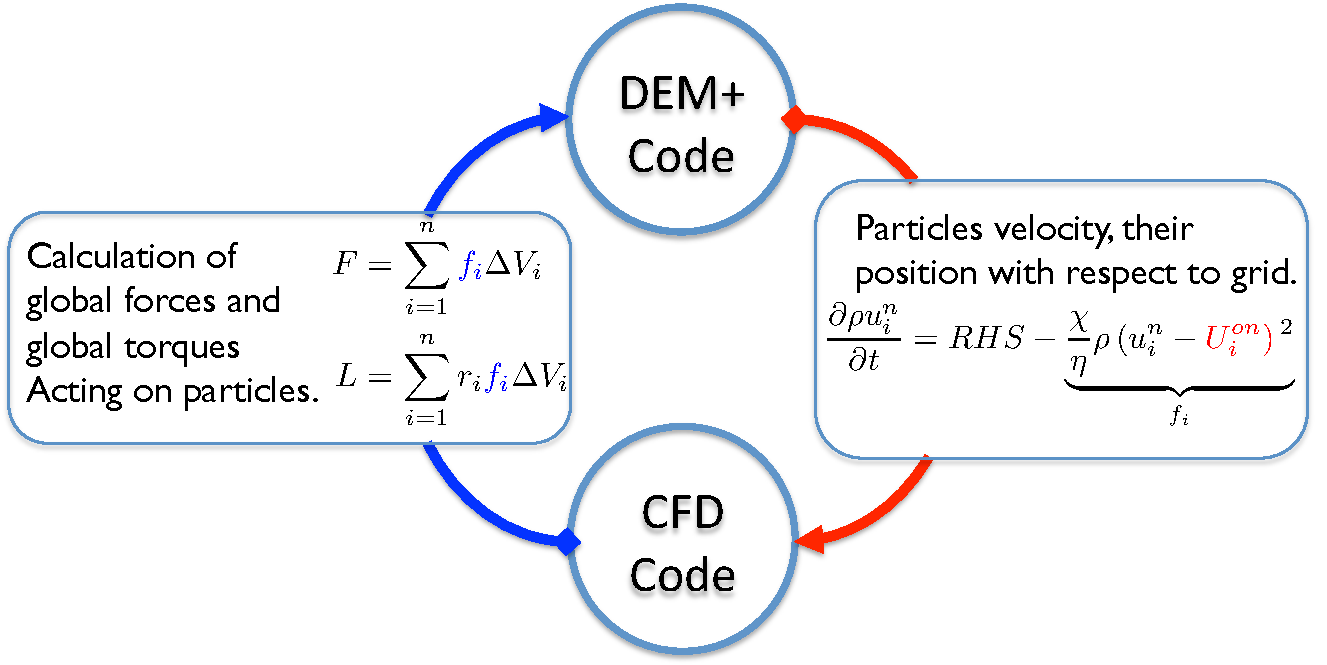
\includegraphics[scale=0.5]{fig/coupling.pdf}\\
\caption{CFD/DEM coupling schematics \label{fig:coupling}}
\end{figure}\\
Set up for all simulations is presented in Fig.~\ref{fig:lofi-domain}. Normal shock with $Ma=5$ approaches either one or multiple ellipsoidal particles in upward direction. Gravitational effects are neglected. Particles either fixed in space or can be driven by the flow, and interact with each other in case of several particles.
\begin{figure}[h!]
\centering 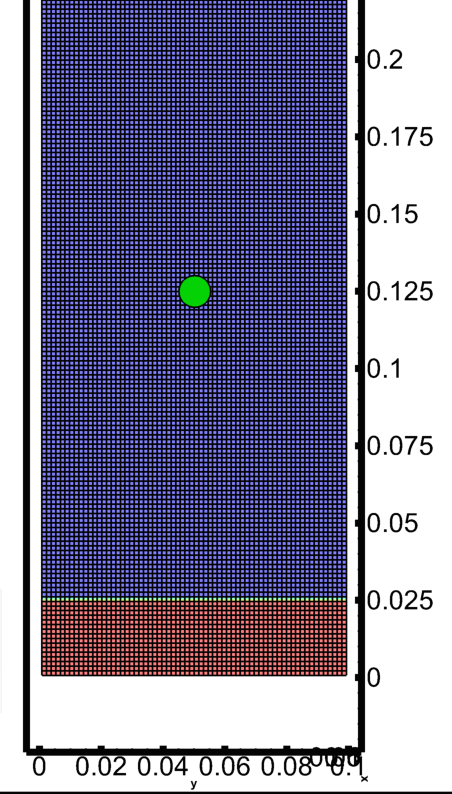
\includegraphics[scale=0.3]{fig/lofi-domain.png}\\
\caption{Low Fidelity simulations set up \label{fig:lofi-domain}}
\end{figure}\\
Simulations were carried for wide variety of particles of ellipsoidal shape and size by changing values of semi axes for both free and stationary particles.

\section{Flow around Single Stationary Sphere}
For testing purposes VPM was first used for the supersonic flow around fixed spherical particle (see Fig.~\ref{fig:lofi_single_stat}). On the left plot one can find pressure force and penalization force. Latter reaches a plato after shock passes the obstacle since it is stationary and force is proportional to the square of relative velocity according to \eqref{eq:lofi-penal}. Pressure force on the other hand becomes negative since energy equation is not penalized in a consistent way. This issue was resolved in later simulations. Also, one can notice obstacle on the left plot, which has polyhedral shape due to the coarse mesh.
\begin{figure}[t]
\begin{minipage}{0.5\linewidth}
\centering{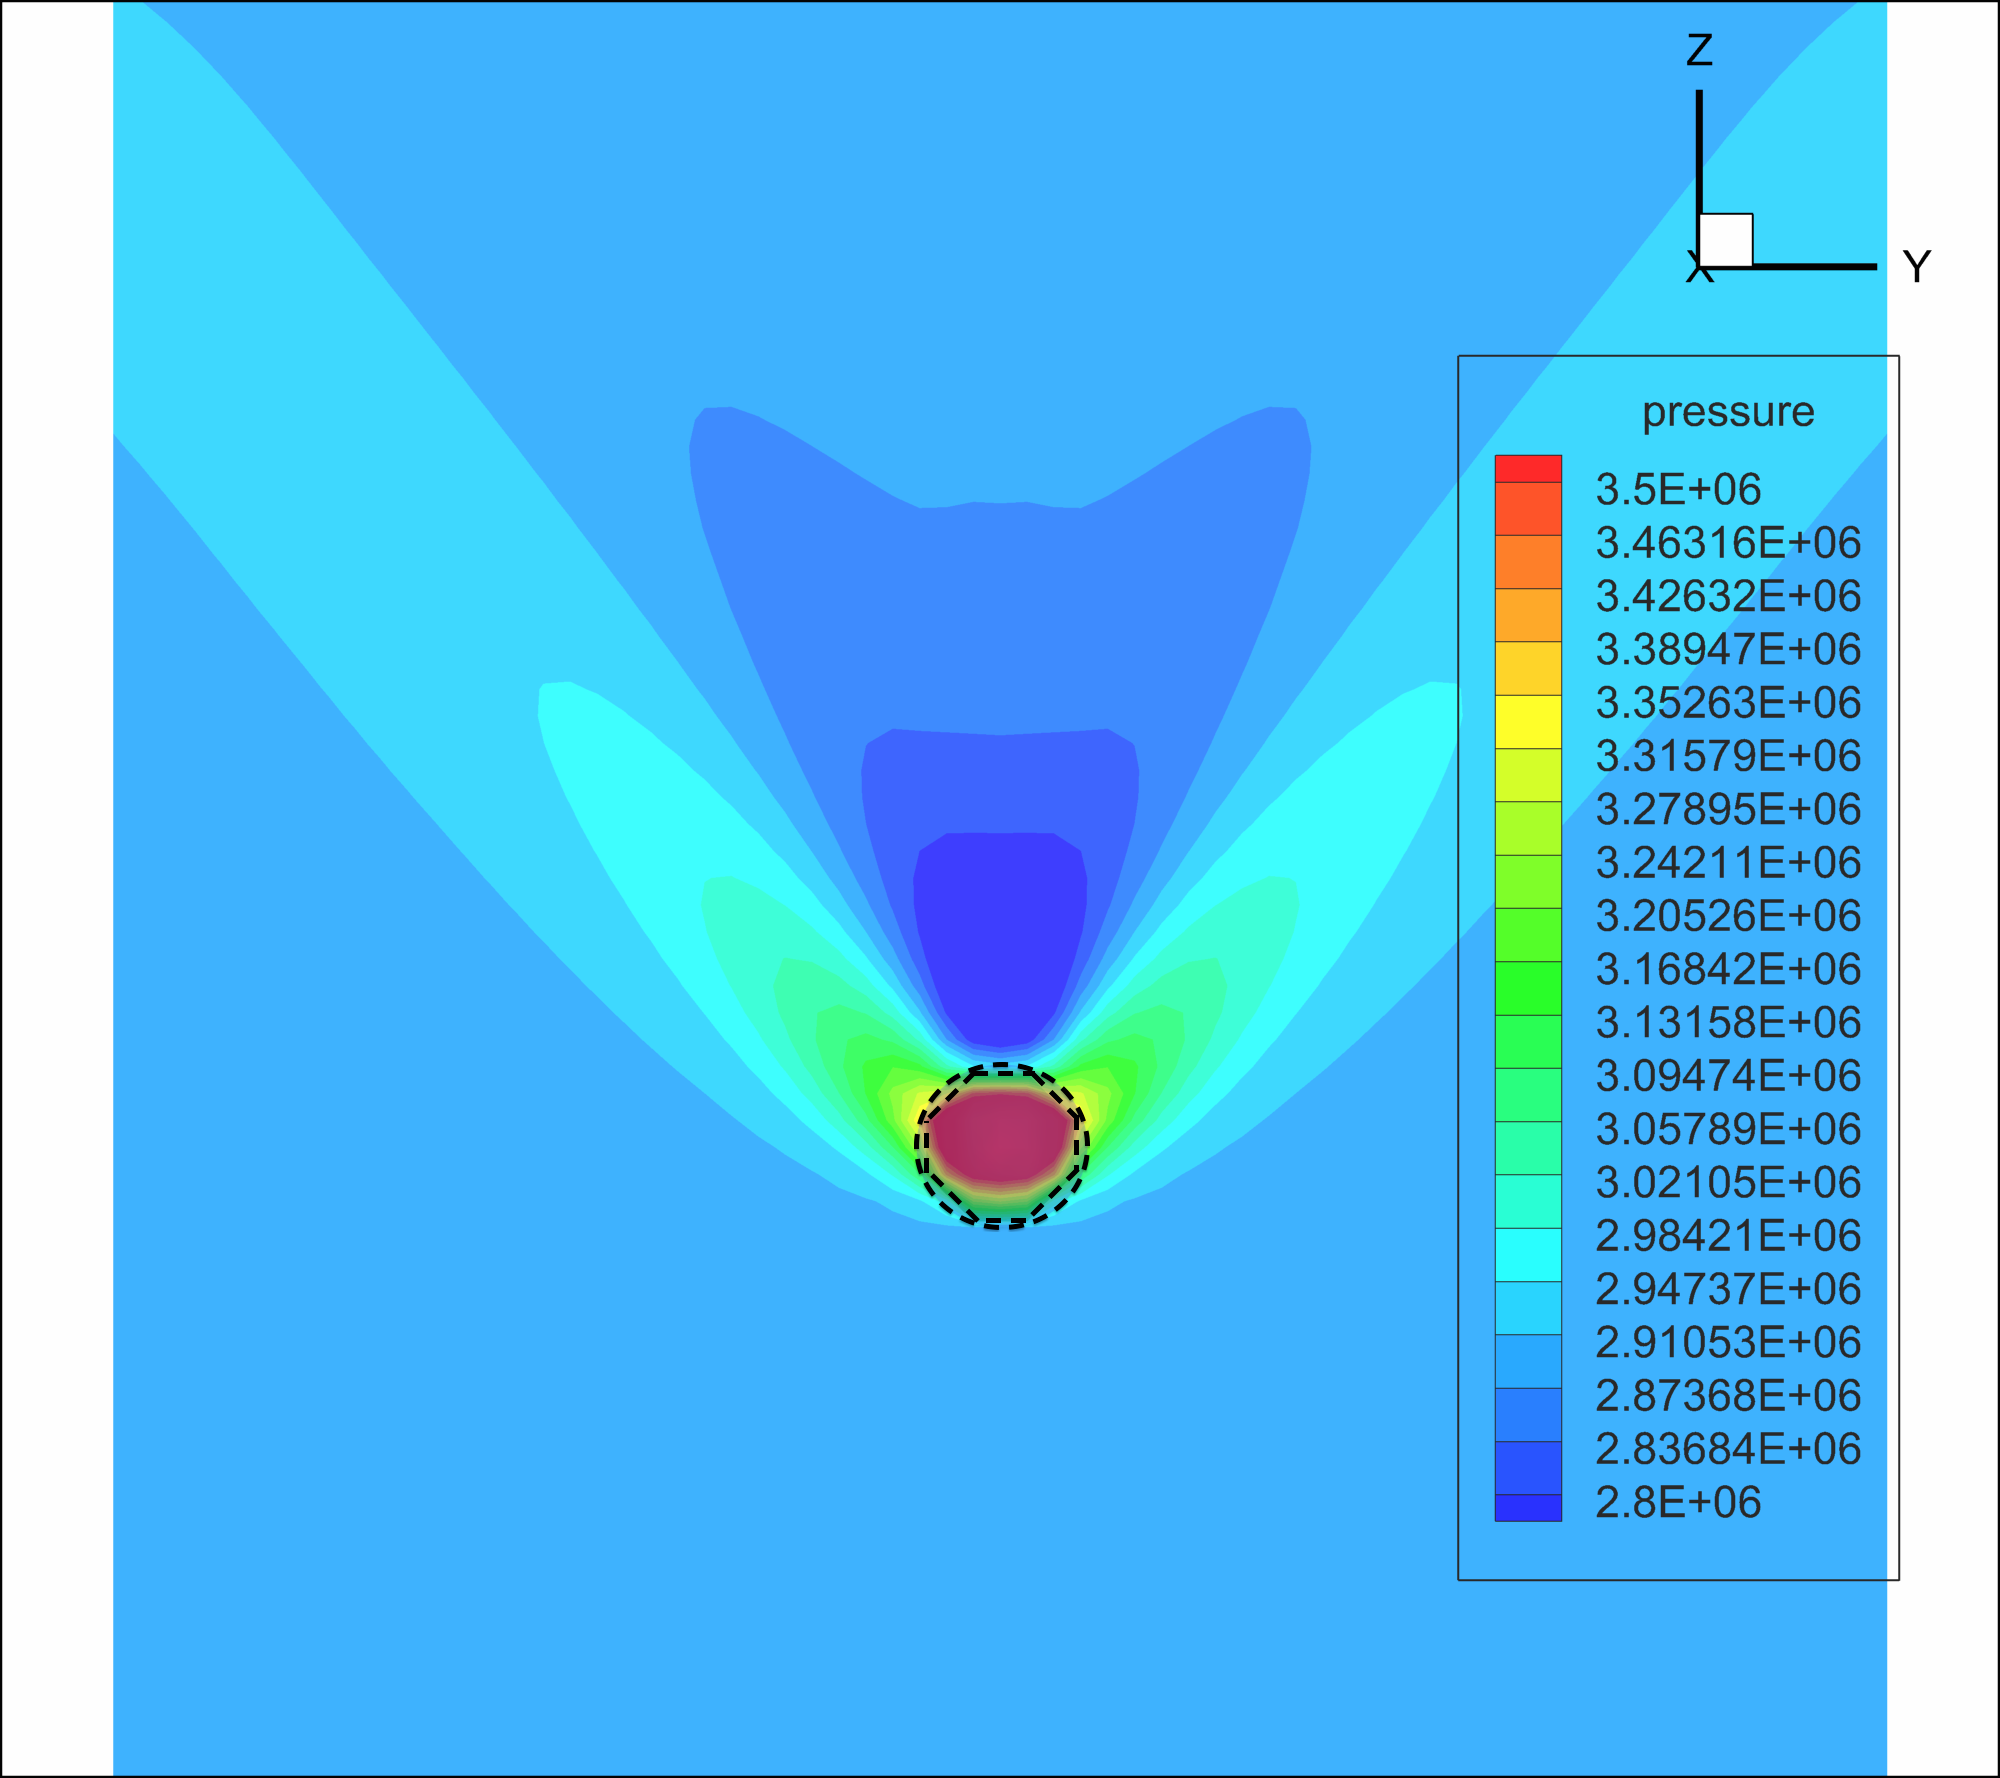
\includegraphics[height=7cm]{fig/lofi_single_stat.png}}
\end{minipage}
\begin{minipage}{0.5\linewidth}
\centering {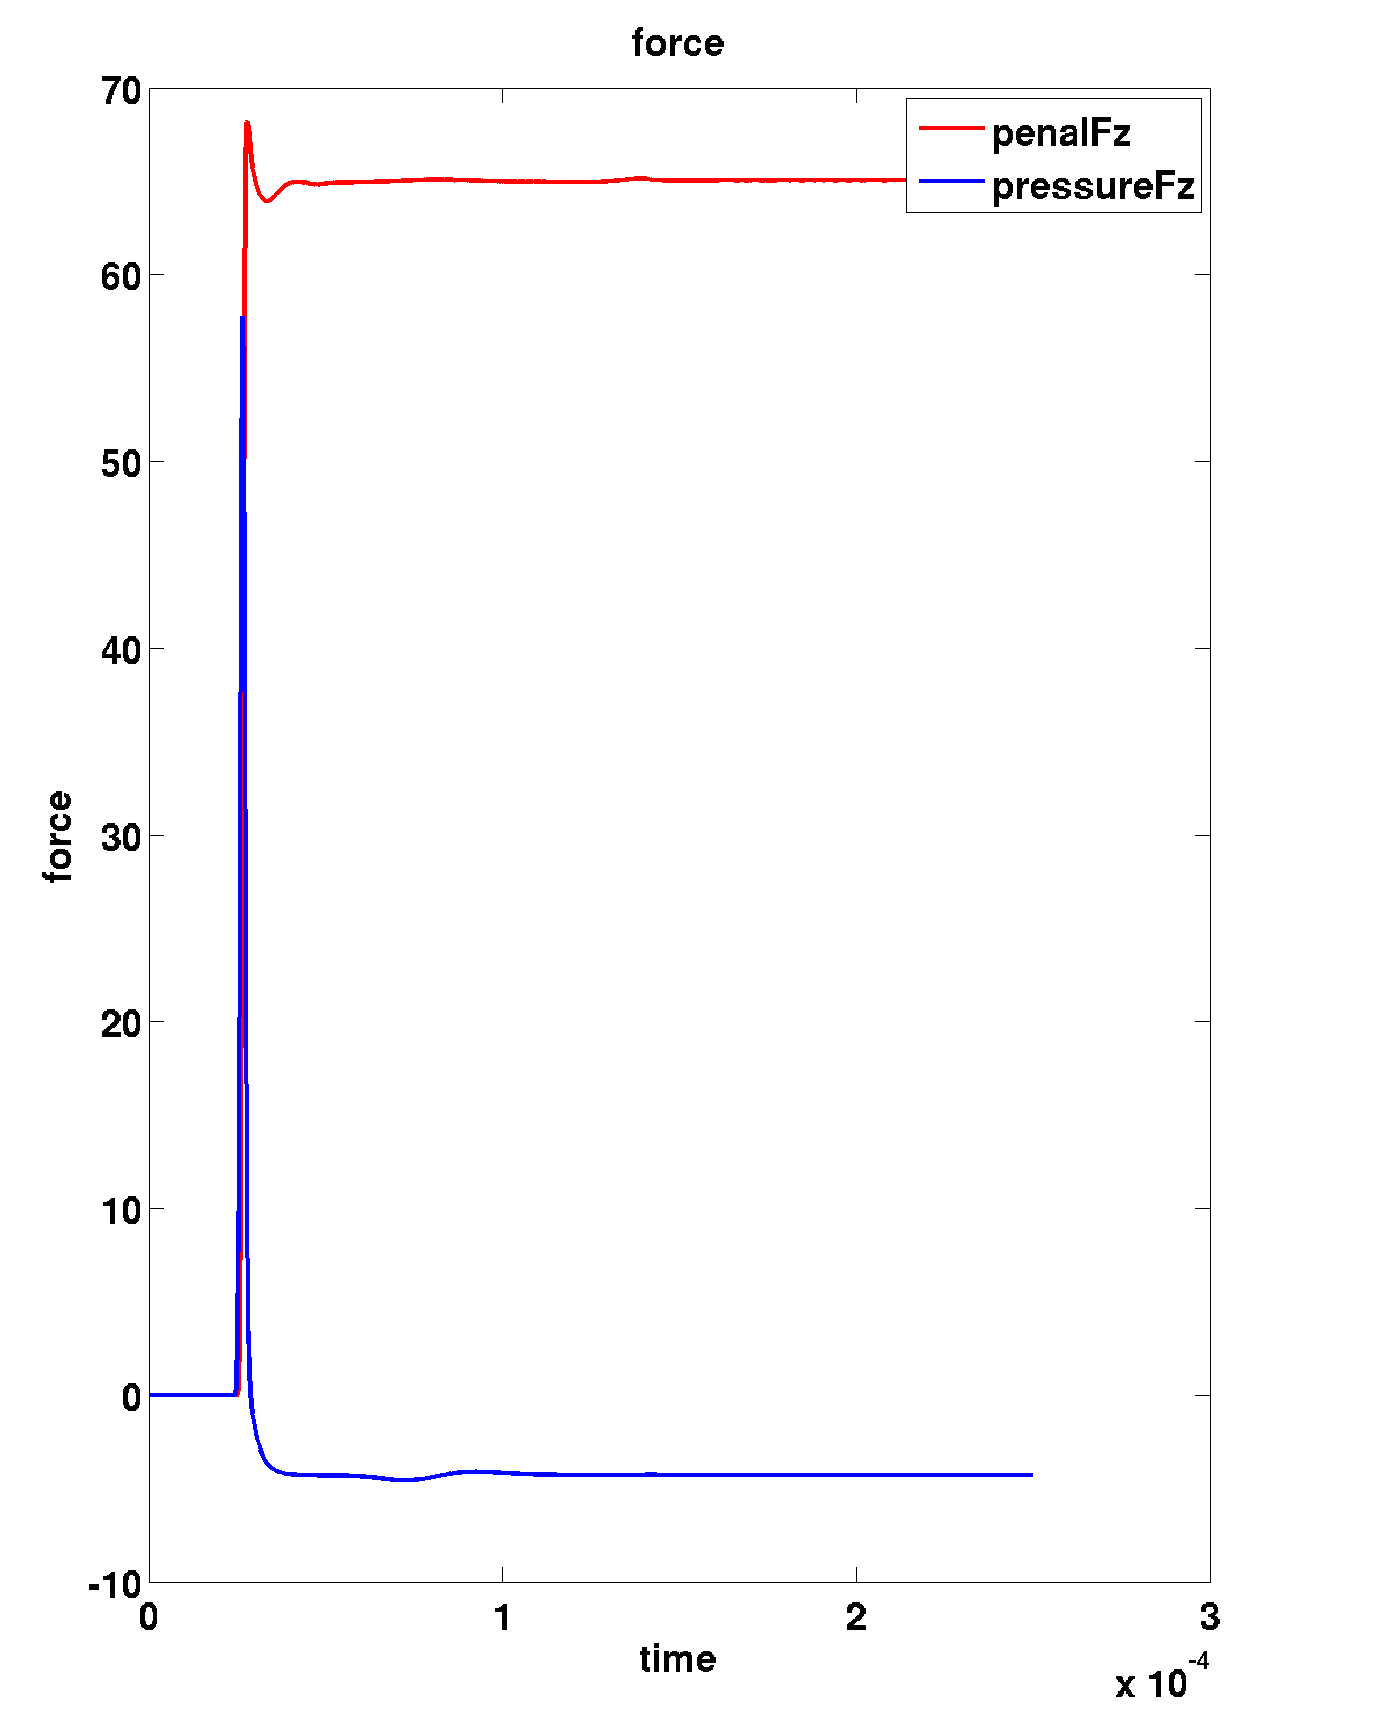
\includegraphics[height=7cm]{fig/lofi_single_force.png}}
\end{minipage}
\caption{Flow around single stationary sphere} \label{fig:lofi_single_stat}
\end{figure}

\section{Flow around Moving Sphere}
Next step in the project is to test the methodology on free spherical particle (see Fig.~\ref{fig:lofi_single_vf}).
\begin{figure}[h!]
\begin{minipage}{0.5\linewidth}
\centering{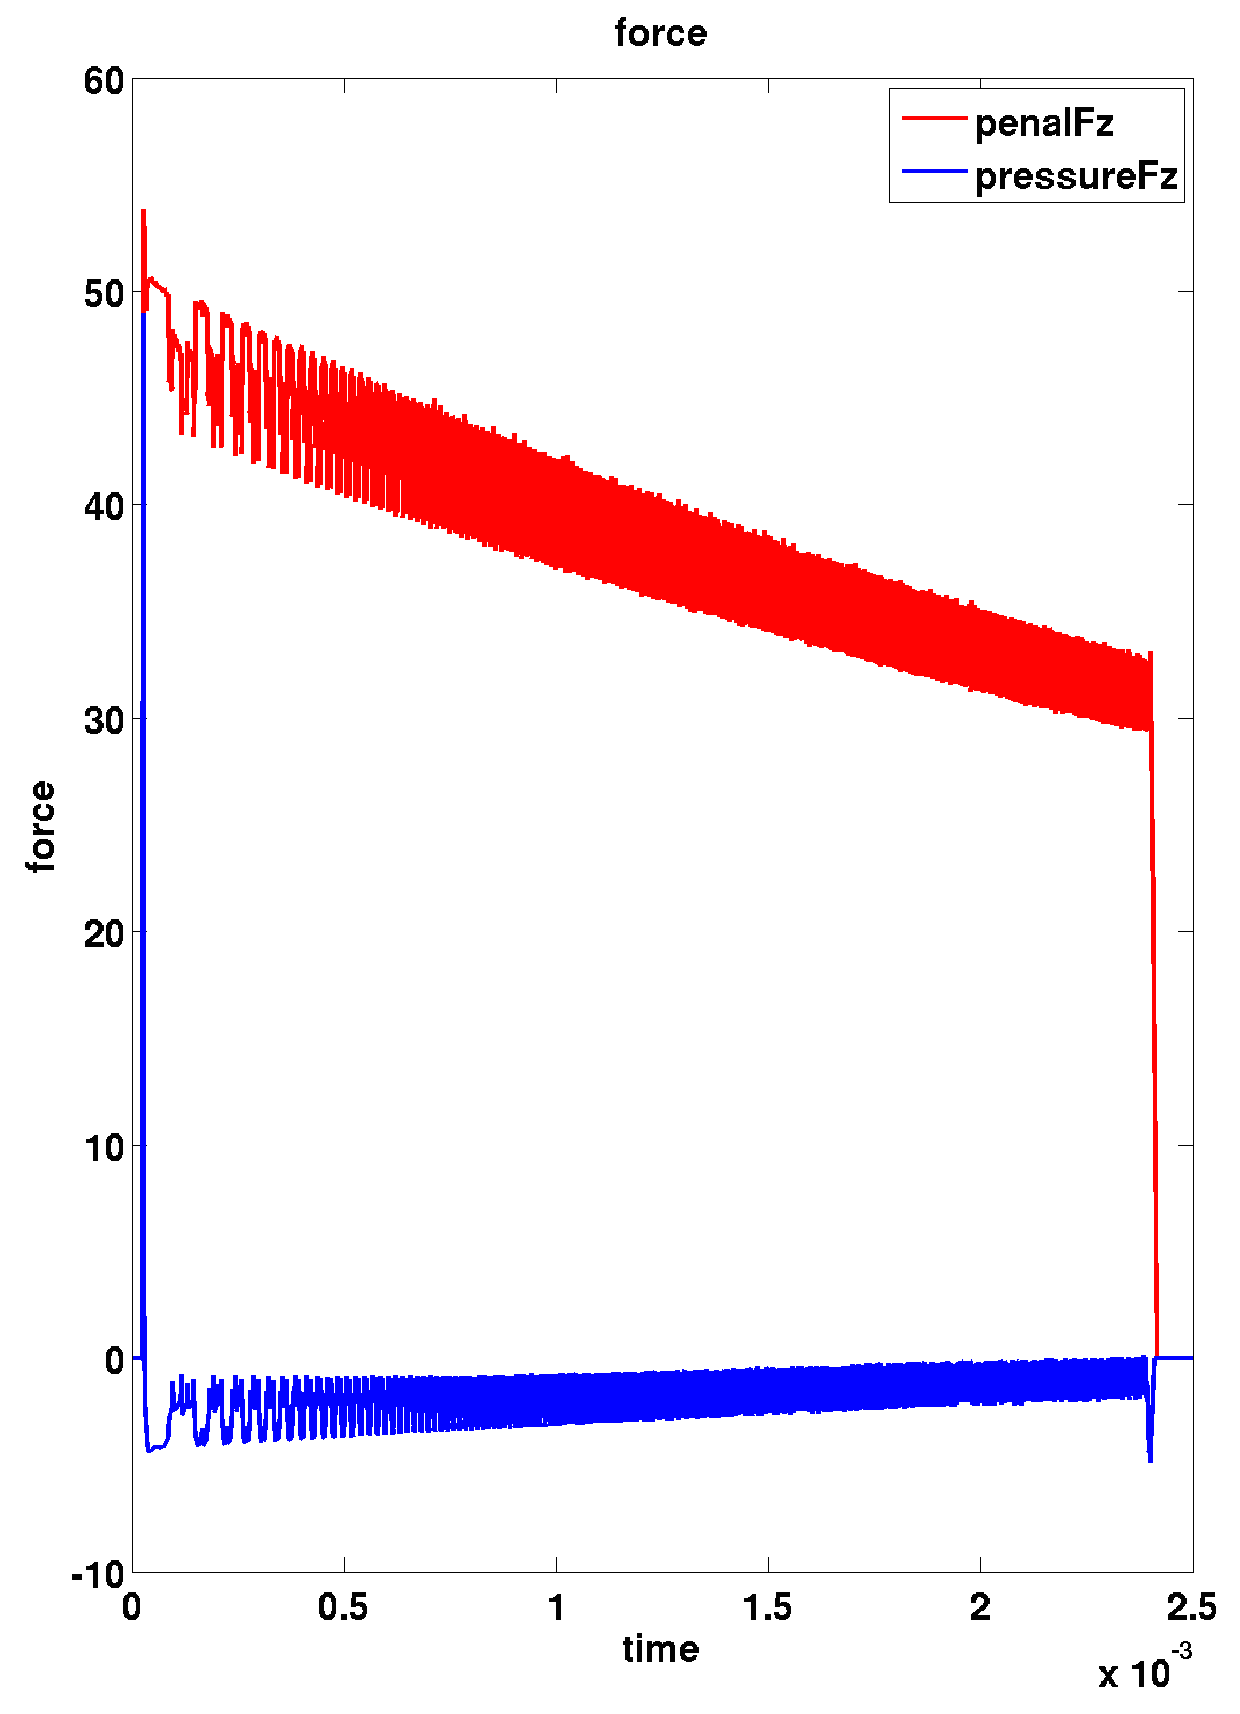
\includegraphics[height=7cm]{fig/lofi_single_novf.png}}
\end{minipage}
\begin{minipage}{0.5\linewidth}
\centering {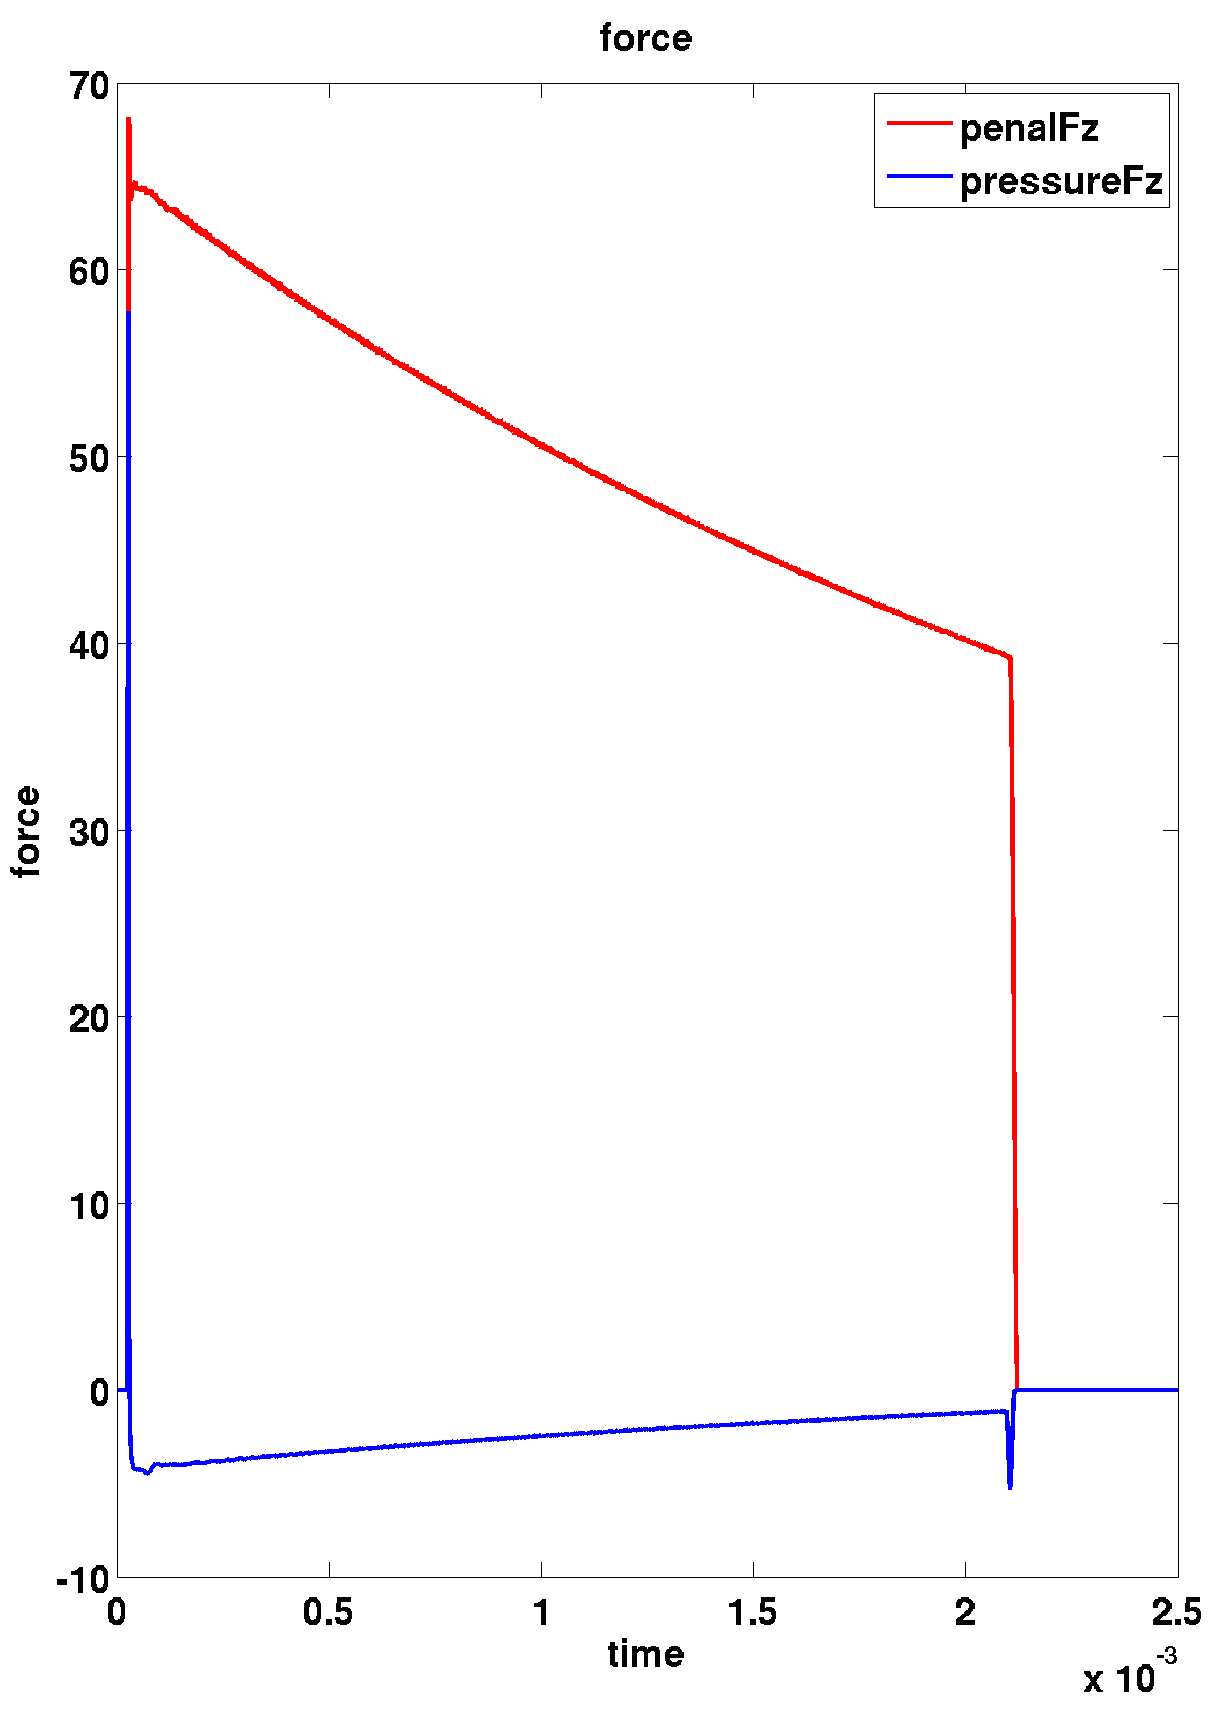
\includegraphics[height=7cm]{fig/lofi_single_vf.png}}
\end{minipage}
\caption{Flow around single free sphere} \label{fig:lofi_single_vf}
\end{figure}\\
On the left plot forces demonstrate noisy behavior. The reason is in coarse grid, so when particle moves the grid cell that particle occupies at any given moment of time might suddenly change when time advances. To solve this issue partial volumes taken by particles are calculated (see Fig.~\ref{fig:lofi-vf}) and results can be found on the right plot. Negative pressure force is still present.
\begin{figure}[h!]
\centering 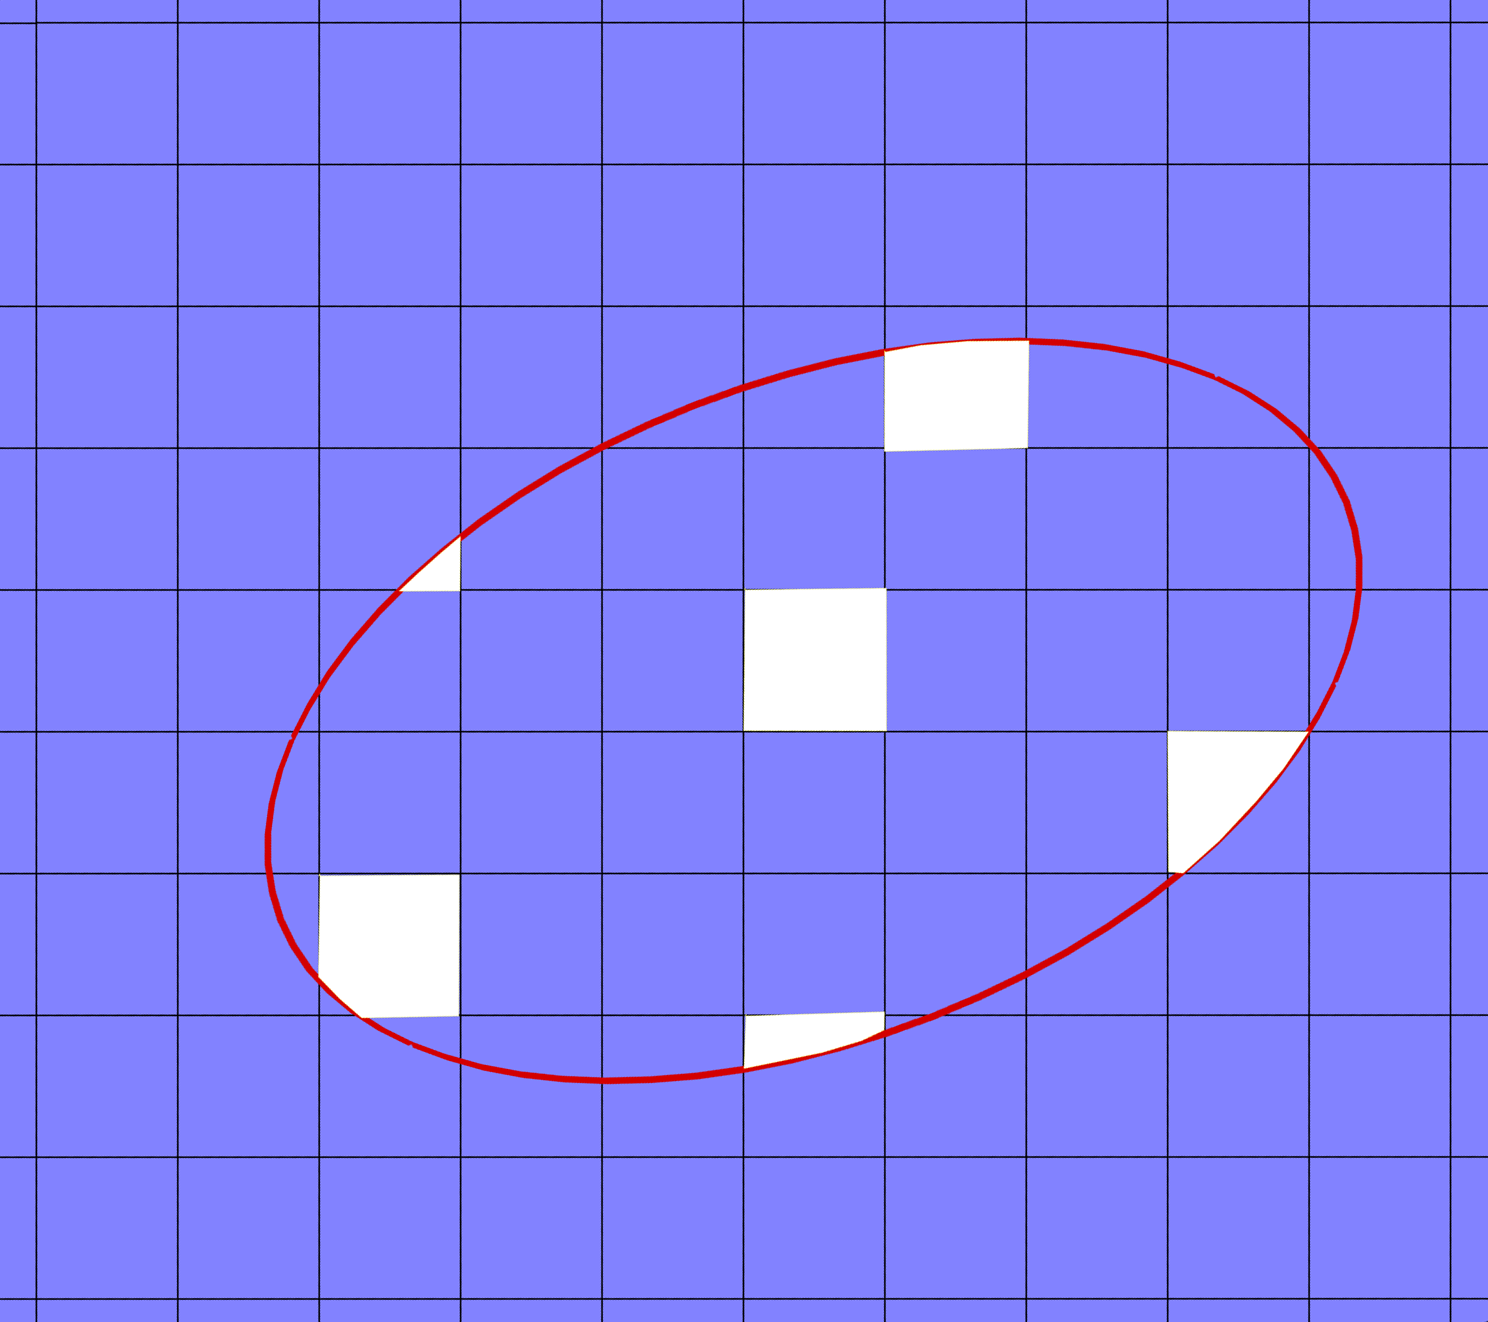
\includegraphics[scale=0.2]{fig/lofi_vf.png}\\
\caption{Grid cells occupied partially by the particle calculated more accurately \label{fig:lofi-vf}}
\end{figure}

\section{Flow around Several Free Ellipsoids}
The method is tested on two and more particles (see Fig.~\ref{fig:lofi_2pt}). During the simulation smaller particle at lower position accelerates more due to the smaller mass and penalization force depends on the relative velocity only. After hitting bigger particle on top it slows down, but later accelerates again. This process continues until both particles stick together. Negative pressure is still present.

In case of substantial number of particles situation changes, instead of going through the particles and forming bow shape shocks as in case of few particles, shock reflects from the wall of particles as if they cannot be penetrated (see Fig.~\ref{fig:lofi_1kpt}).
\begin{figure}[t]
\begin{minipage}{0.5\linewidth}
\centering{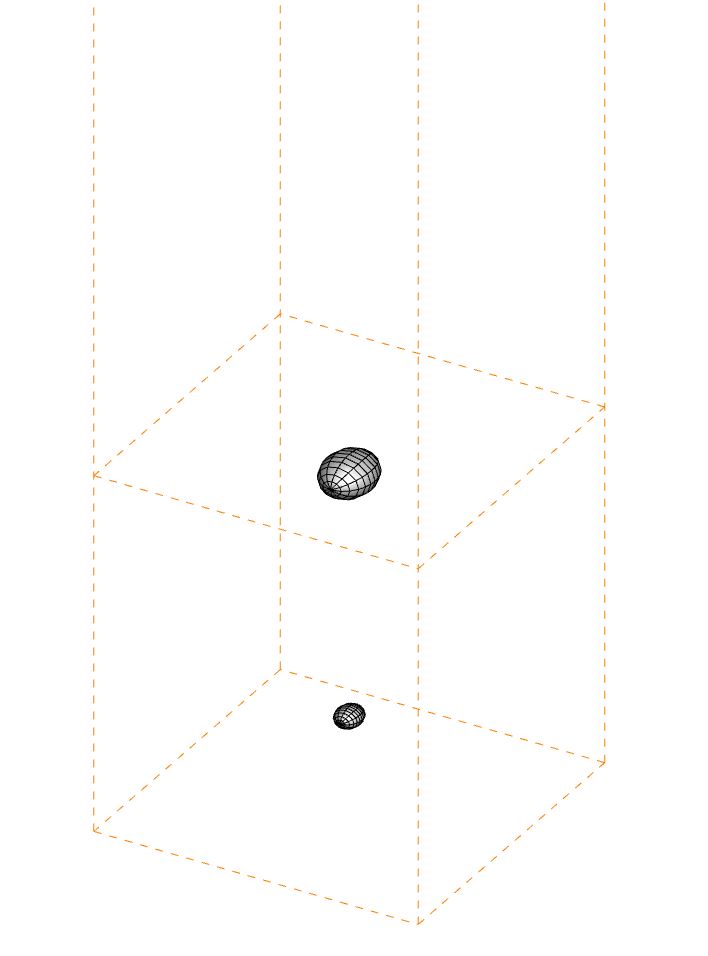
\includegraphics[height=7cm]{fig/lofi_2pt.png}}
\end{minipage}
\begin{minipage}{0.5\linewidth}
\centering {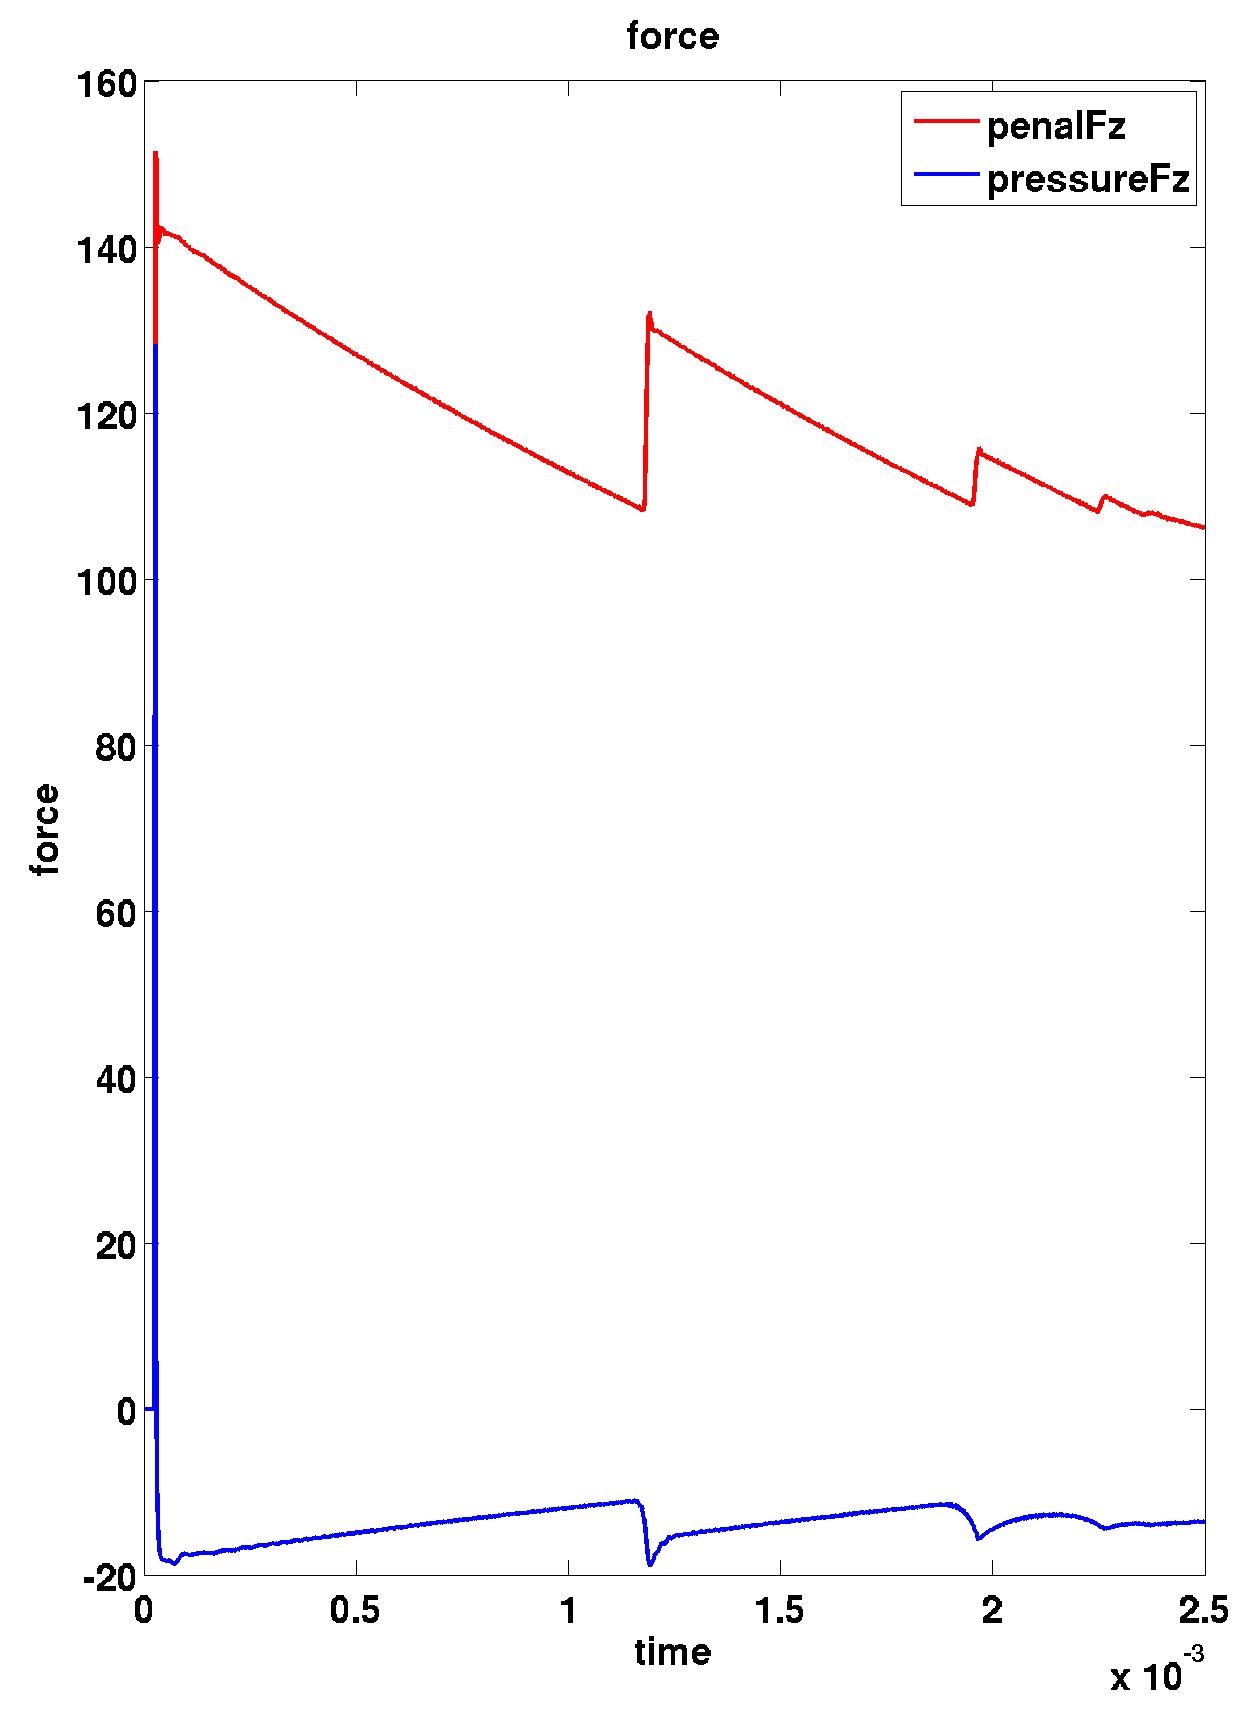
\includegraphics[height=7cm]{fig/lofi_2pt_force.png}}
\end{minipage}
\caption{Flow around two ellipsoidal particles} \label{fig:lofi_2pt}
\end{figure}
\begin{figure}[h!]
\begin{minipage}{0.5\linewidth}
\centering{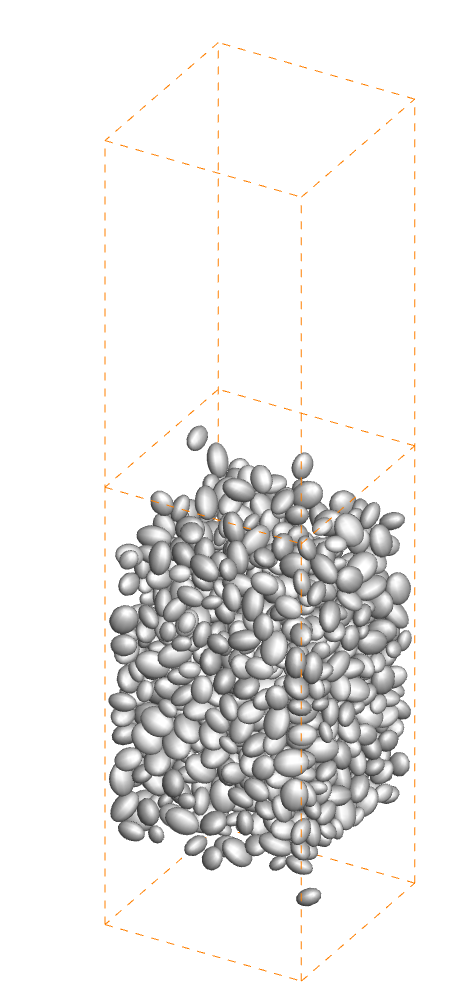
\includegraphics[height=7cm]{fig/lofi_many_pts.png}}
\end{minipage}
\begin{minipage}{0.5\linewidth}
\centering {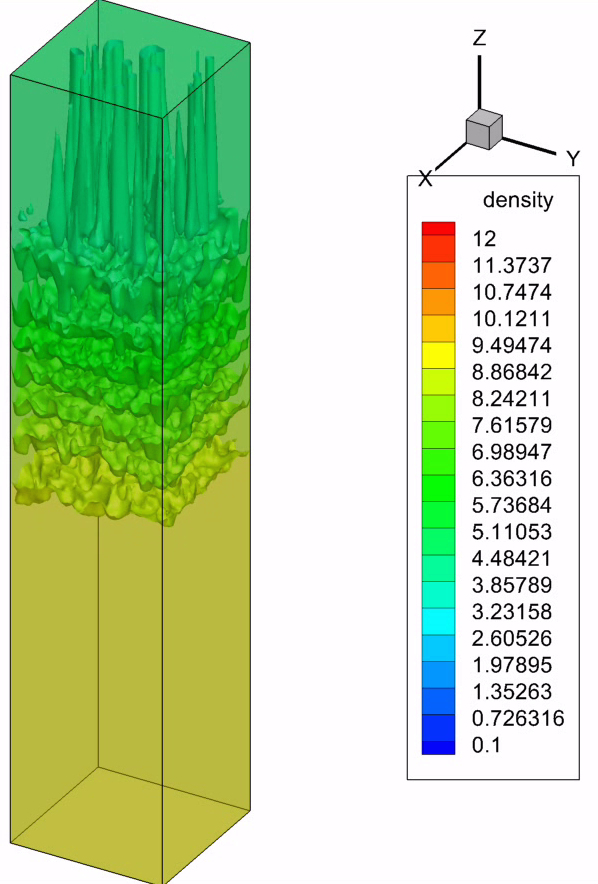
\includegraphics[height=7cm]{fig/lofi_many_den.png}}
\end{minipage}
\caption{Flow around 1k ellipsoidal particles} \label{fig:lofi_1kpt}
\end{figure}

\section{Flow around ``Disk'' and ``Needle'' like obstacles}
Ellipsoidal, and potentially polyellipsoidal, particles have a flexibility of imitating different shapes. For example, by squeezing one of the semi axis and having other two approximately equal to each other one can get disk shape particle. By squeezing two semi axis and keeping third one relatively large one can imitate needle like object (see Fig.~\ref{fig:lofi_shapes}).
\begin{figure}[t]
\begin{minipage}{0.5\linewidth}
\centering{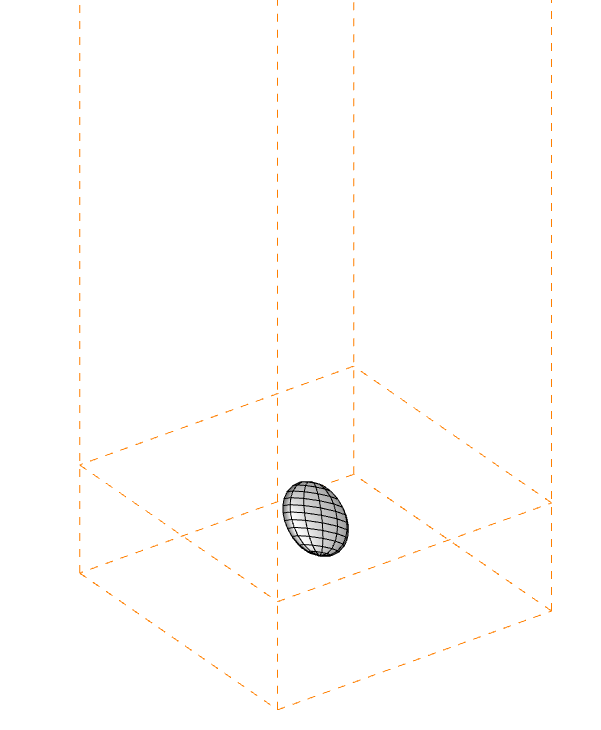
\includegraphics[height=7cm]{fig/lofi_disk.png}}
\end{minipage}
\begin{minipage}{0.5\linewidth}
\centering {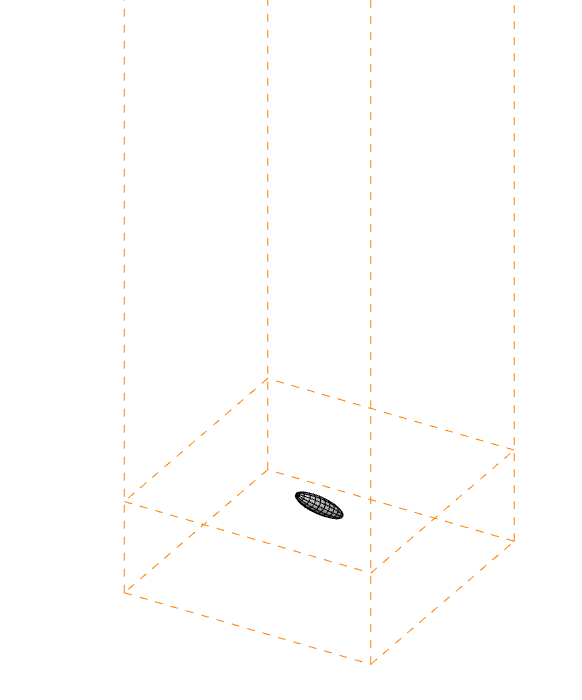
\includegraphics[height=7cm]{fig/lofi_needle.png}}
\end{minipage}
\caption{Disk shape (left) and needle shape (right) particles} \label{fig:lofi_shapes}
\end{figure}
\begin{figure}[h!]
\begin{minipage}{0.5\linewidth}
\centering{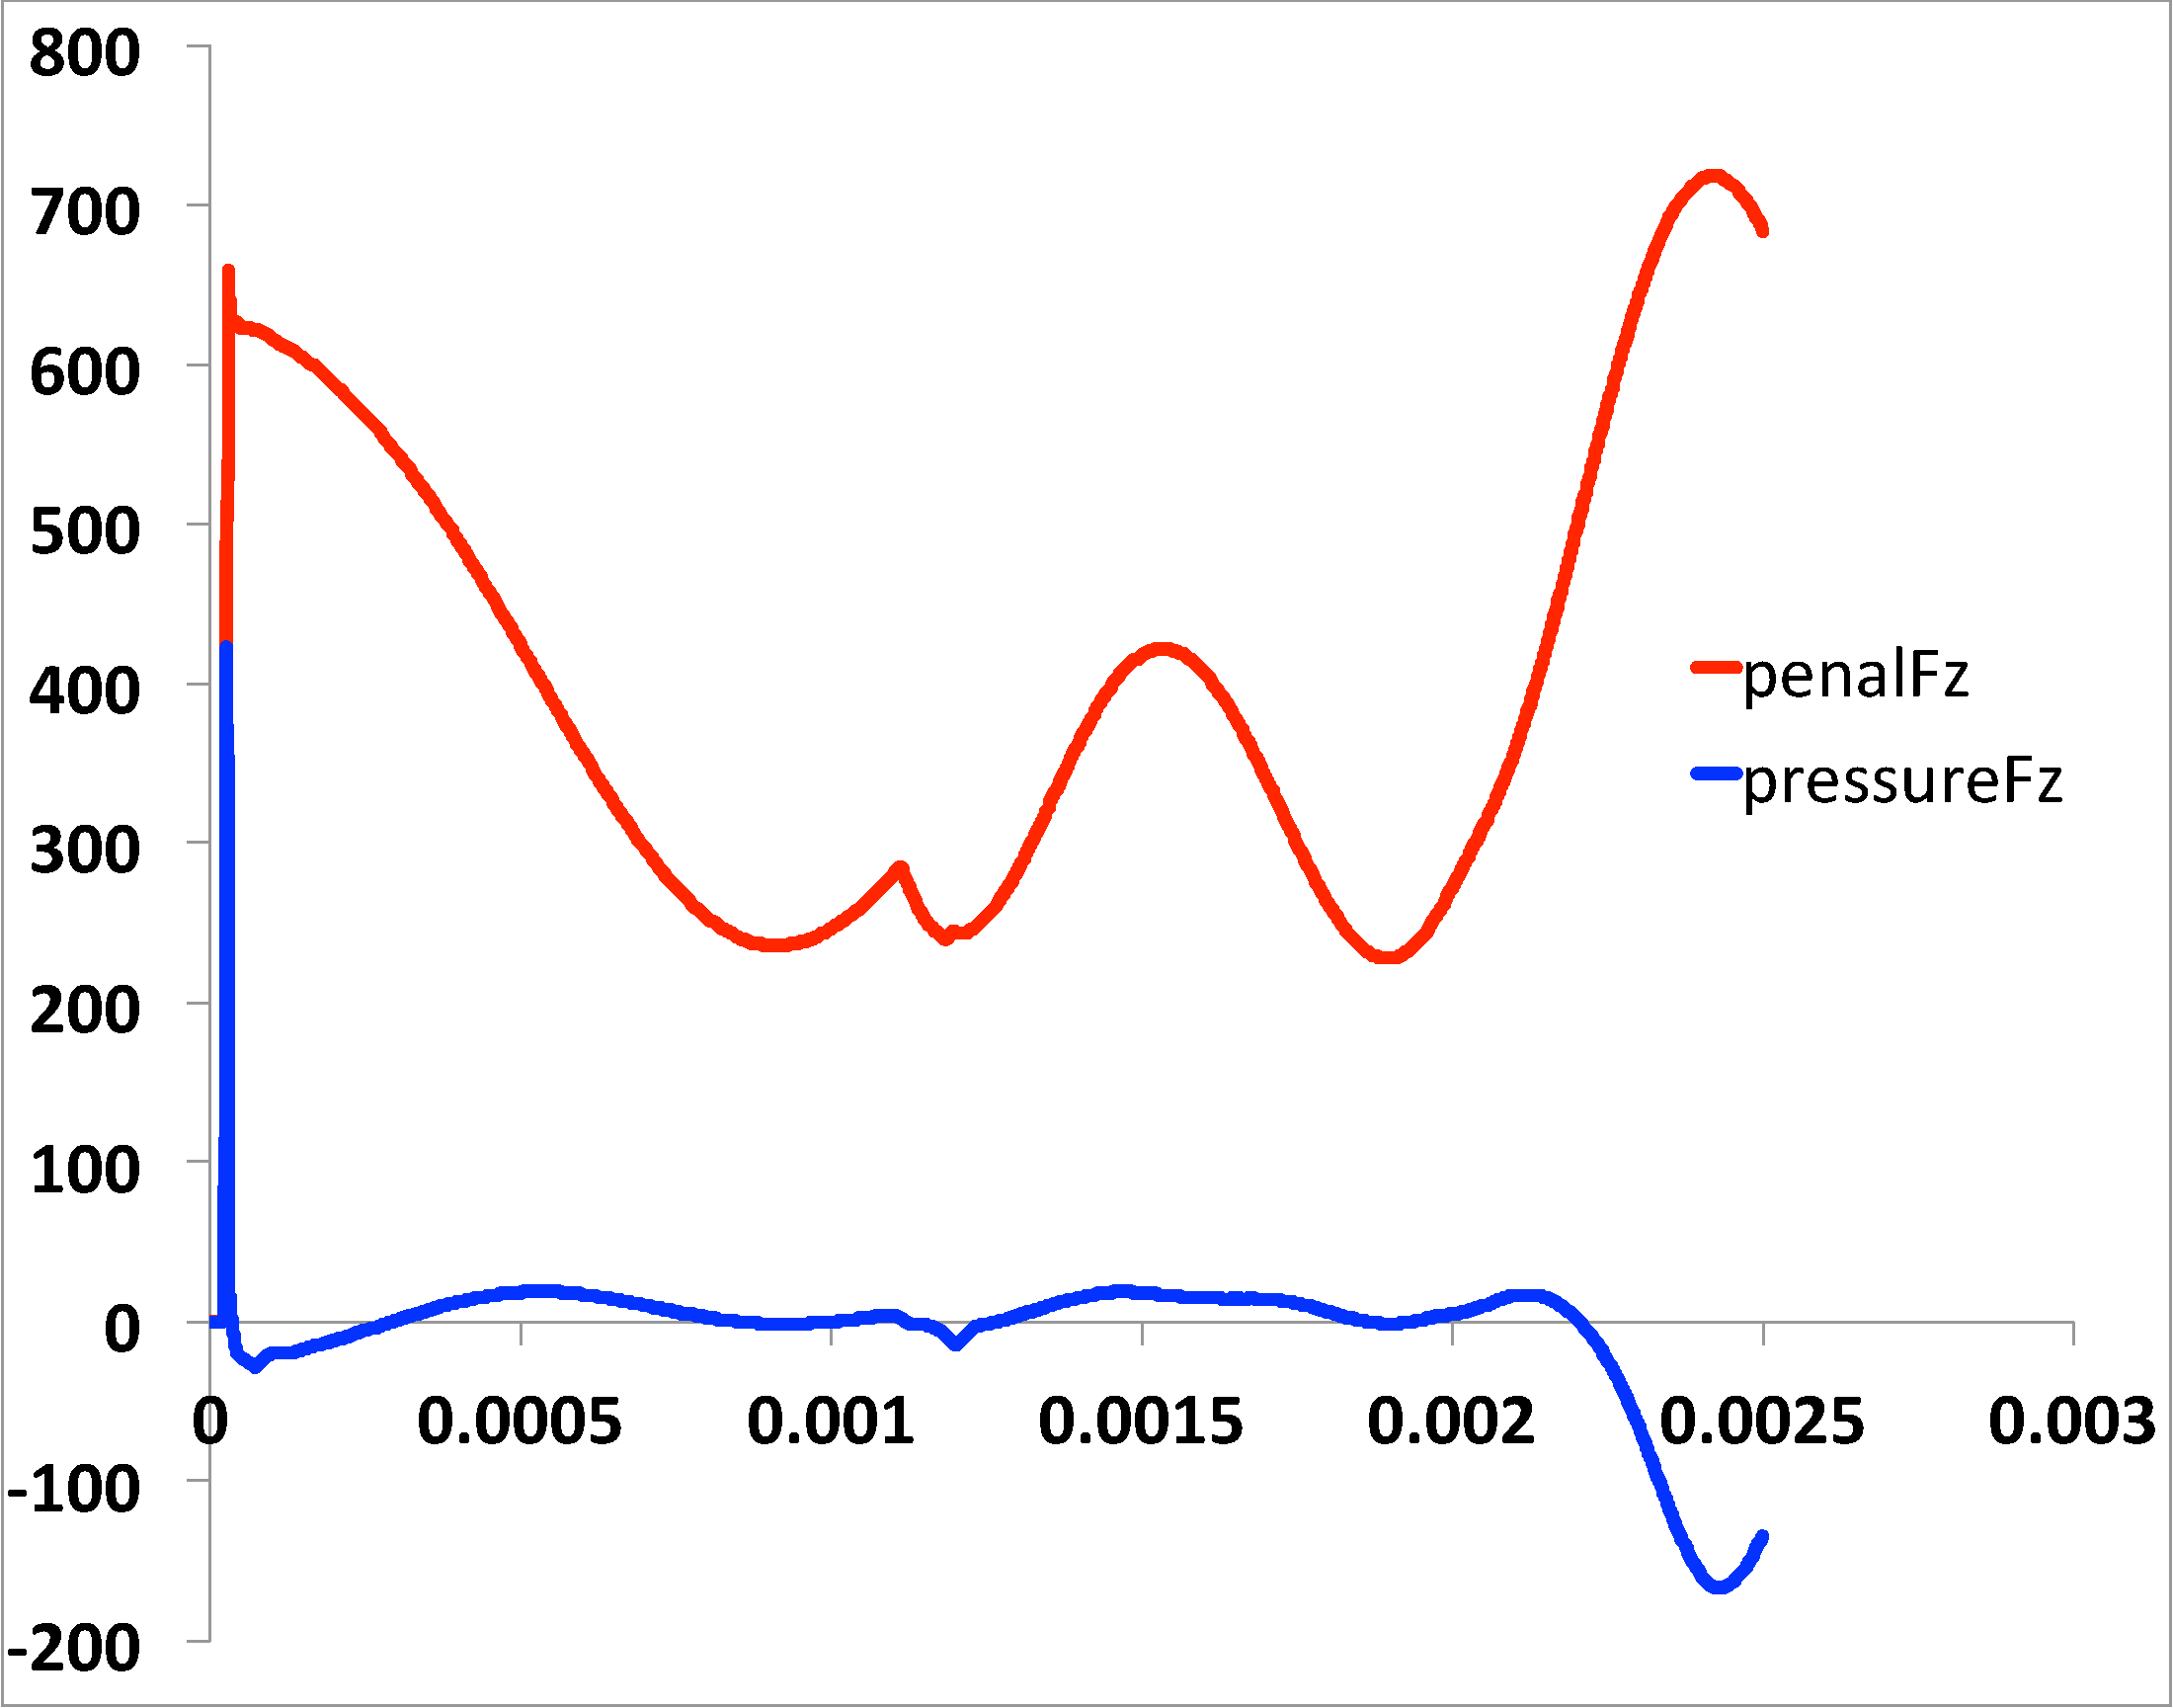
\includegraphics[height=5.5cm]{fig/lofi_disk_force.pdf}}
\end{minipage}
\begin{minipage}{0.5\linewidth}
\centering {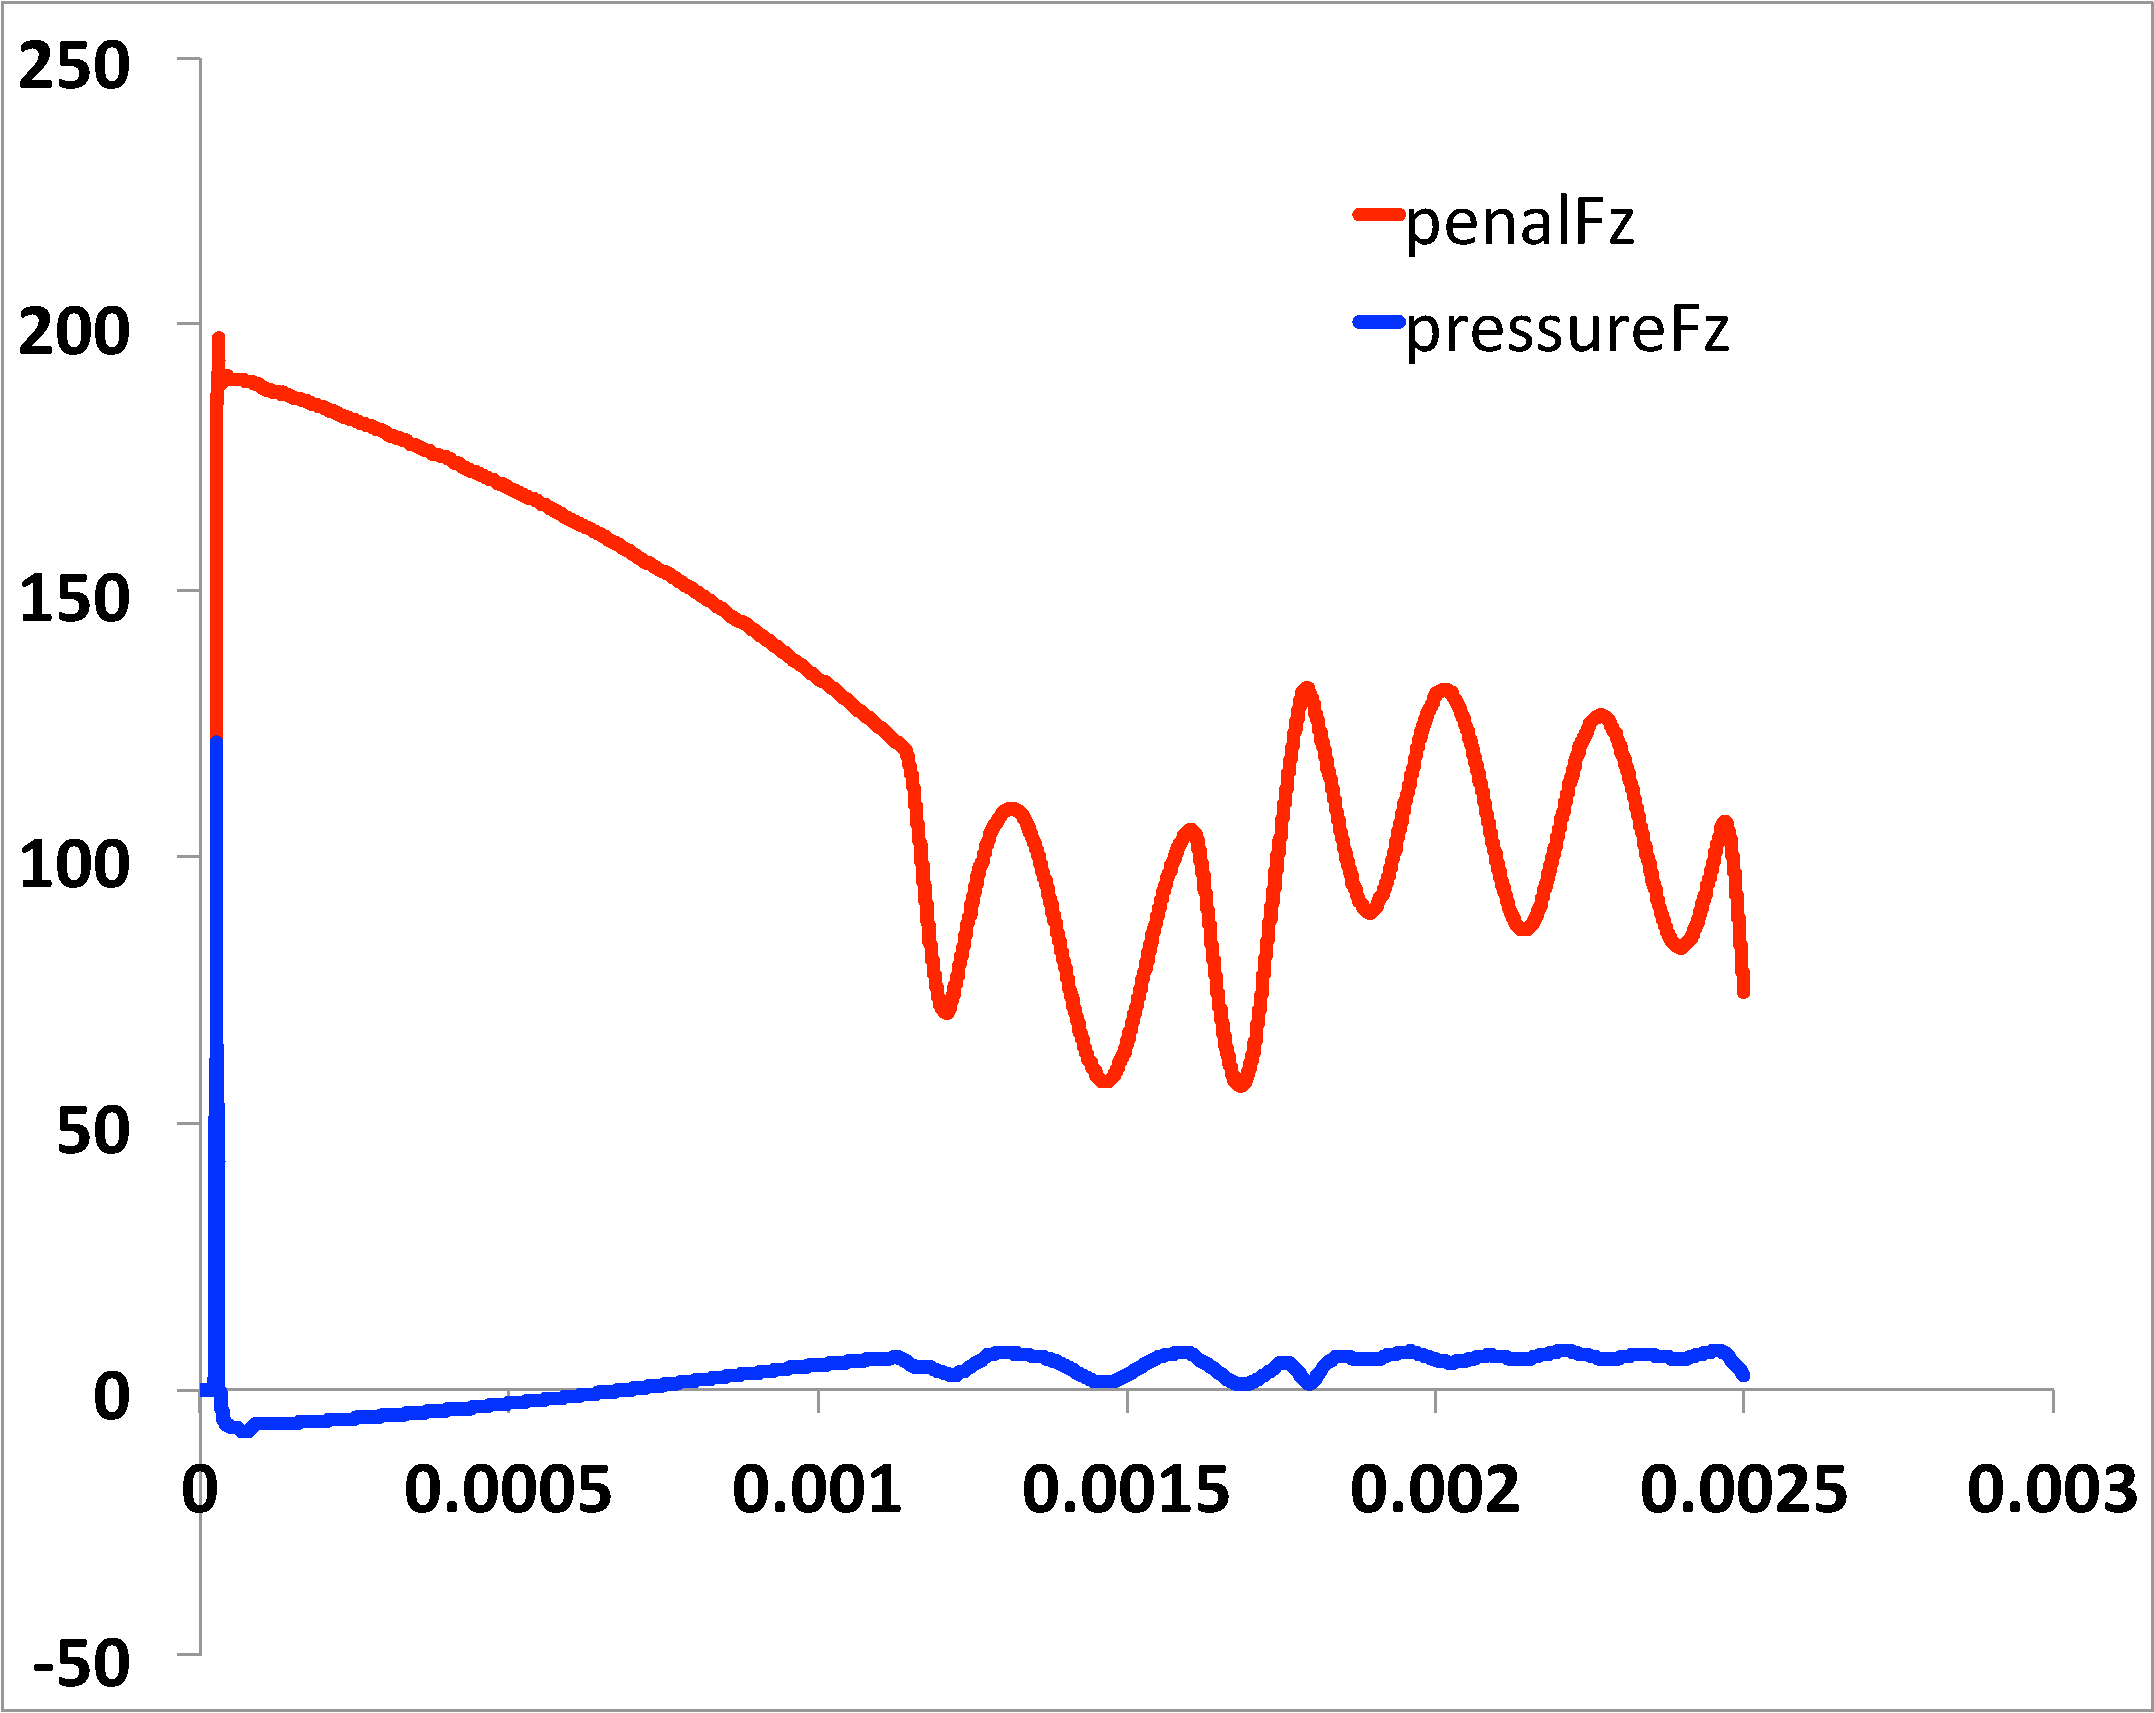
\includegraphics[height=5.5cm]{fig/lofi_needle_force.pdf}}
\end{minipage}
\caption{Dynamics of the flow around disk (left) and needle (right)} \label{fig:lofi_shapes_force}
\end{figure}\\
From results, one can see that penalization force oscillates at some point. The reason is particles bounce from vertical sides of the domain loosing energy (see Fig.~\ref{fig:lofi_shapes_force}). Negative pressure is still present.

\section{Flow around Stationary Ellipsoid, Negative Pressure Fix}
One can notice that all previous simulations have negative pressure issue. In order to fix it more accurate penalization is chosen (see Fig.~\ref{fig:lofi_single_fix}). It reproduces density penalization according to \eqref{eq:poro_den} and energy penalization according to \eqref{eq:CBVP_euler}. Latter is necessary step, since it makes equations consistent with each other, but former is meant to take into account the fact that despite small penalization parameter $\eta$ that acts like permeability, fluid penetrates to the particle and in case of big particle or large amount of particles, error might become significant.
\begin{figure}[h!]
\centering 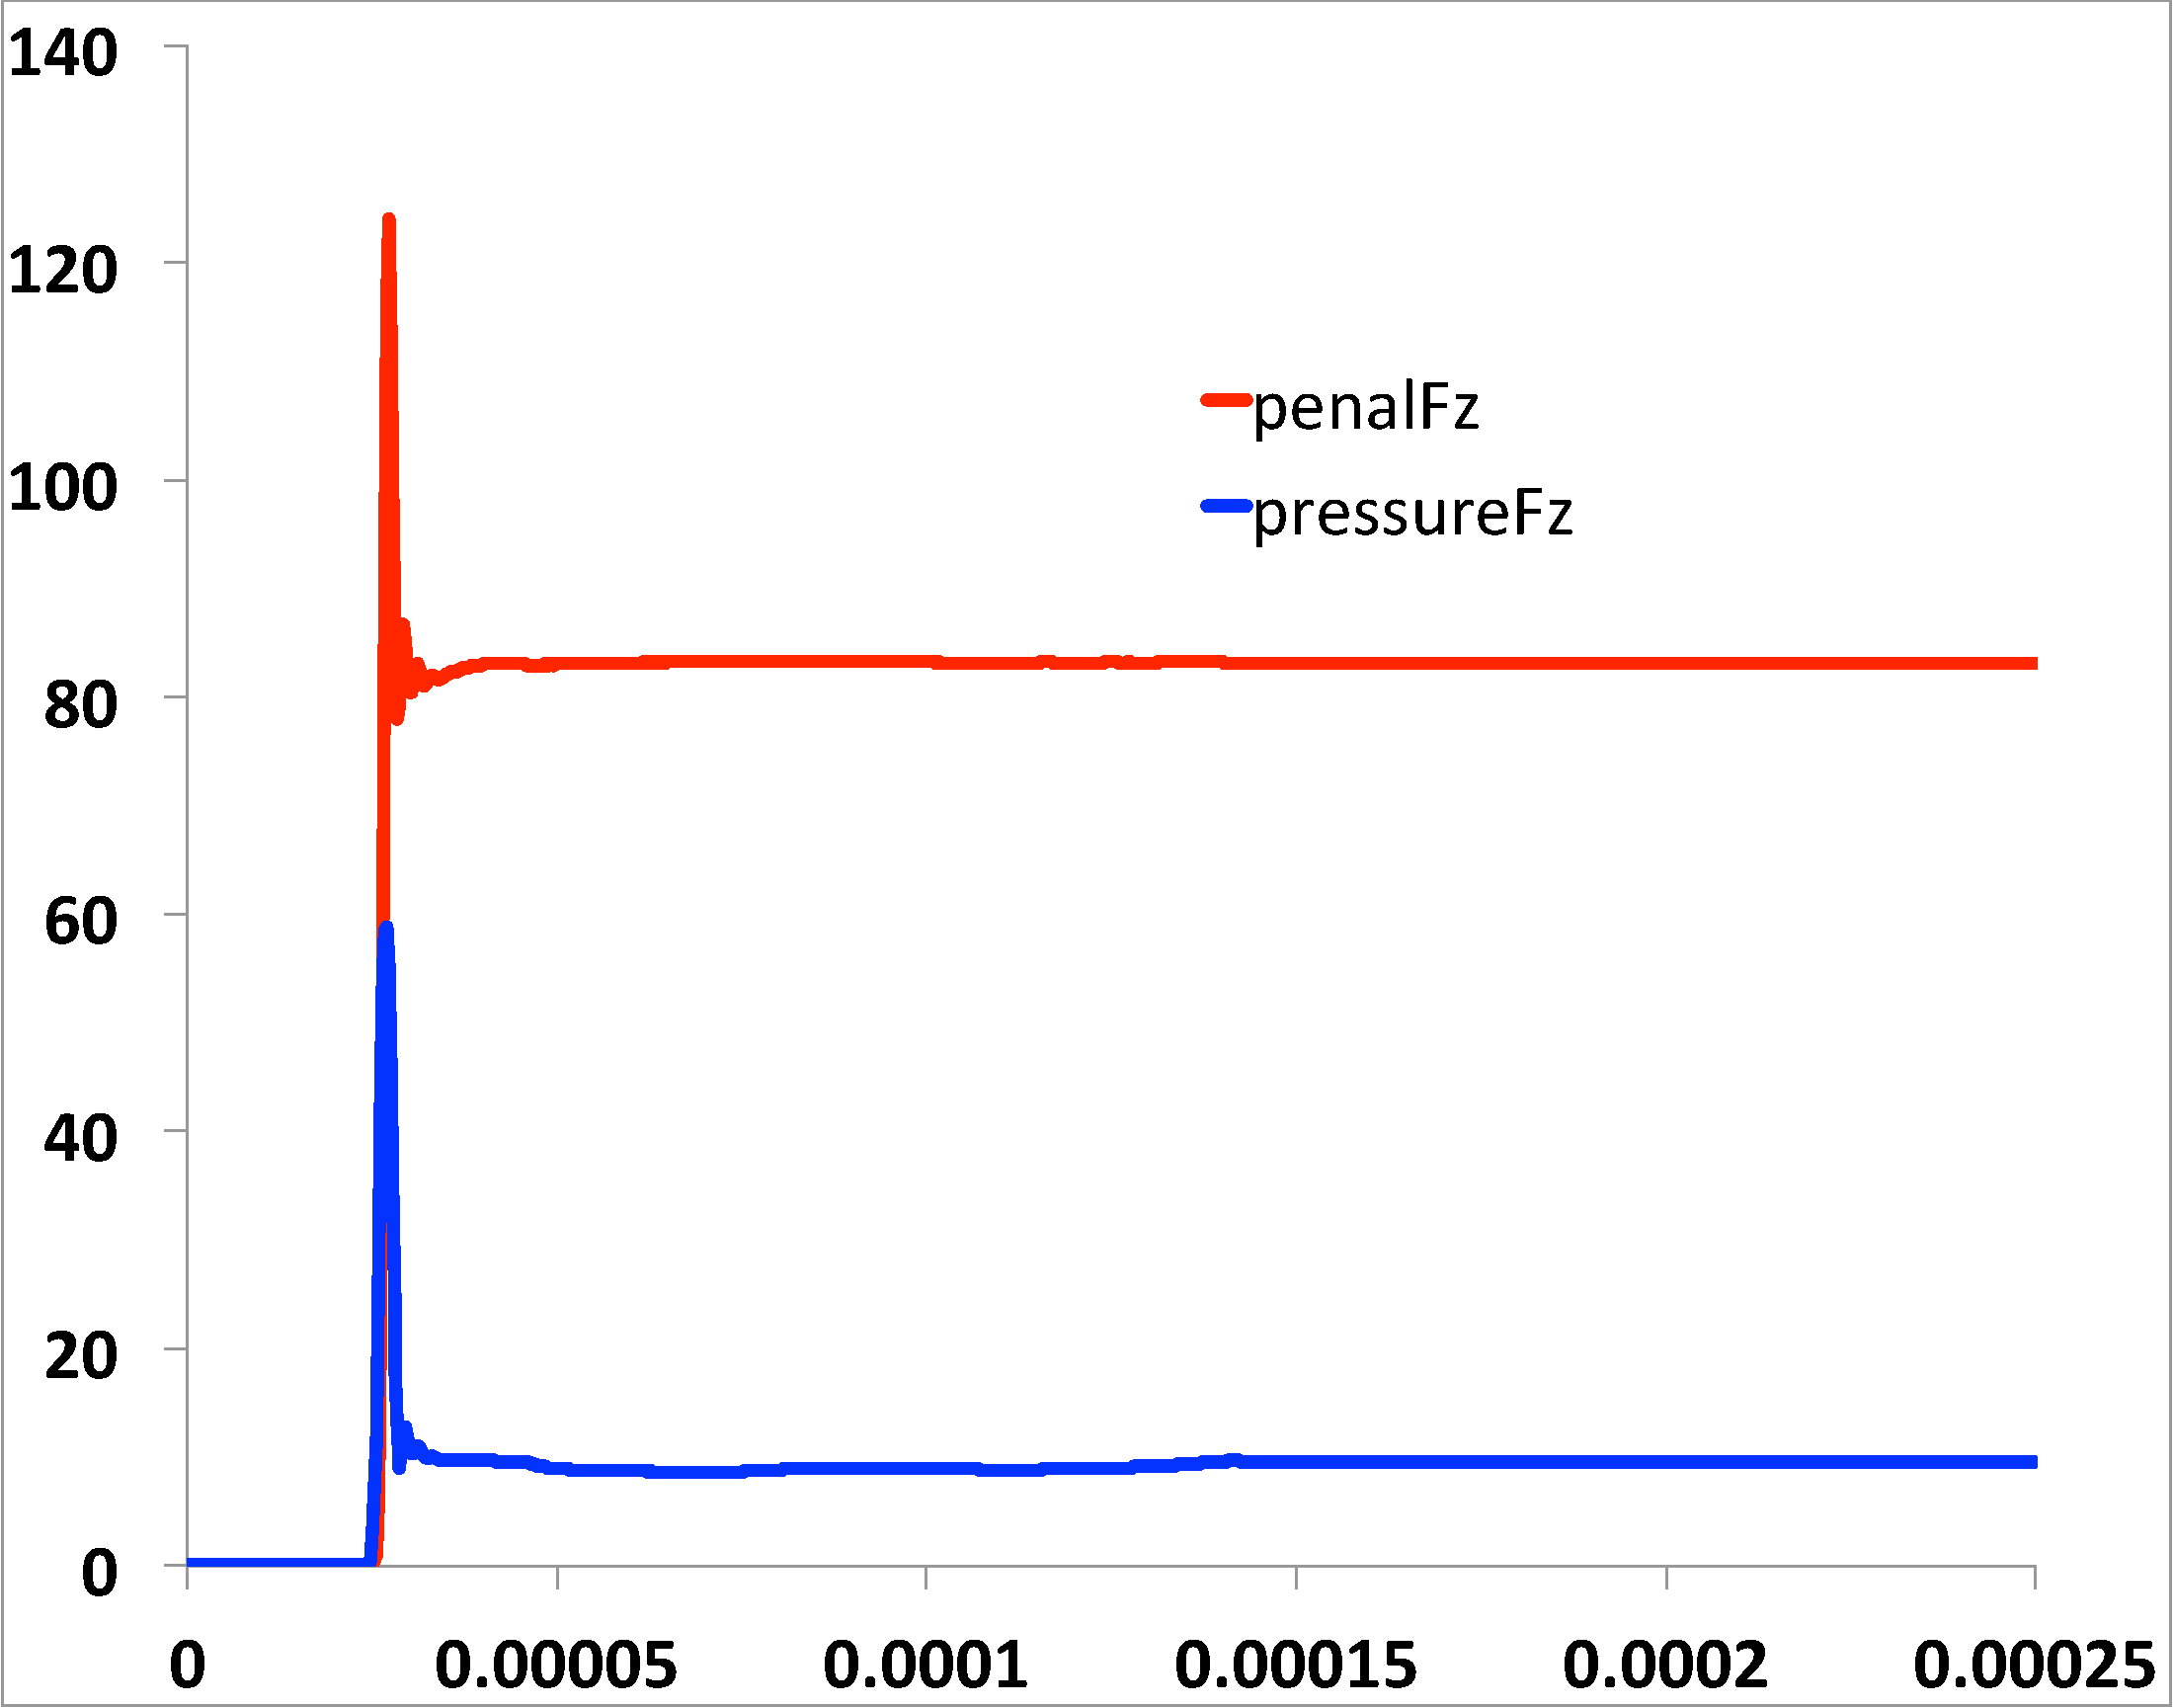
\includegraphics[scale=0.2]{fig/lofi_single_fix.pdf}\\
\caption{Flow around single ellipsoid with porosity fix and energy fix  enabled \label{fig:lofi_single_fix}}
\end{figure}